\documentclass[11pt,DIV=11]{scrartcl}
\usepackage[utf8]{inputenc}
\usepackage[english]{babel}
\usepackage[ruled]{algorithm2e}
\usepackage{aligned-overset}
\usepackage{alltt}
\usepackage{amsmath}
\usepackage{amsthm}
\usepackage{csquotes}
\usepackage{enumerate}
\usepackage{multicol}
\usepackage{stmaryrd}
\usepackage{subcaption}
\usepackage{xcolor}

% \setlength\parskip{0.2em}
\binoppenalty=32767
\relpenalty=32767

\def\code#1{\texttt{\frenchspacing#1}}
\def\padding{\vspace{3em}}

\usepackage{tikz}
\tikzstyle{node}=[fill=white, draw=black, shape=circle, minimum size=2em]
\tikzstyle{blue node}=[fill=white, draw=blue, shape=circle]
\tikzstyle{red node}=[fill=white, draw=red, shape=circle]
\tikzstyle{blue edge}=[-, draw=blue]
\tikzstyle{red edge}=[-, draw=red]
\tikzstyle{dashed edge}=[-, dashed]
\pgfdeclarelayer{nodelayer}
\pgfdeclarelayer{edgelayer}
\pgfsetlayers{nodelayer,edgelayer}

\newtheorem{theorem}{Theorem}[section]
\newtheorem{corollary}{Corollary}[theorem]
\newtheorem{lemma}[theorem]{Lemma}
\theoremstyle{definition}
\newtheorem{definition}[theorem]{Definition}
\newtheorem{example}{Example}[theorem]
\theoremstyle{remark}
\newtheorem*{remark}{Remark}

\usepackage[sorting=ynt,style=alphabetic]{biblatex}
\addbibresource{sources.bib}

\title{Sorting by Reversals}
\author{Jonas Hübotter}

\begin{document}

\maketitle

\begin{abstract}
    A reversal is a transformation, reversing the order of elements of a permutation. Sorting by Reversals is the problem of finding the shortest sequence of reversals transforming a permutation to the identity. The length of such a sequence is said to be the reversal distance of that permutation. In this paper we introduce fundamental concepts used in the literature on this topic. In particular, the fundamental relationship between the reversal distance and the number of alternating cycles in a cycle decomposition of a suitably-defined bi-colored graph. Then a $3/2$-approximation is discussed in detail. We also reference further related research.
\end{abstract}

\section{Introduction}

In computational biology a fundamental problem is to identify the evolutionary similarity between genome sequences. By far the most common mutation on genomes is the inversion. A genome can be represented by a permutation. An inversion then simply is the reversal of the substring of a permutation \cite{Kececioglu1995}.

We refer by $\langle S_n, \circ \rangle$ to the symmetric group with $S_n = \{(\pi_1\ \dots\ \pi_n) \mid \{\pi_1, \dots, \pi_n\} = [1,n]\}$. Let $\pi \in S_n$ be a permutation and $\pi_i$ denote $\pi(i)$. The identity permutation $id = (1\ \dots\ n)$ is the permutation mapping every input to itself. A \textit{reversal} $\rho(i,j)$ inverses the substring from $\pi_i$ to $\pi_j$ of a permutation. It is represented by the permutation
\begin{align*}
    (1\ \cdots\ i-1\ j\ j-1\ \cdots\ i+1\ i\ j+1\ \cdots\ n).
\end{align*}
Composing $\pi$ with $\rho(i,j)$ yields $(\pi_1\ \cdots\ \pi_{i-1}\ \pi_j\ \pi_{j-1}\ \dots\ \pi_{i+1}\ \pi_i\ \pi_{j+1}\ \cdots\ \pi_n)$ where the elements $\pi_i, \dots, \pi_j$ have been reversed.

Motivated by the outlined application in computational biology, we define the following problem.

\begin{definition}
Given two permutations $\sigma$ and $\tau$, the \textit{reversal distance problem} is the problem of finding the shortest sequence of reversals transforming $\sigma$ into $\tau$. More formally, we want to find reversals $\rho_1, \dots, \rho_d$ such that
\begin{align*}
    \sigma \circ \rho_1 \circ \cdots \circ \rho_d = \tau
\end{align*}
and $d$ is minimal.
The number of necessary reversals $d$ is called the \textit{reversal distance} between $\sigma$ and $\tau$.
\end{definition}

We now observe that the very same shortest sequence of reversals transforming $\sigma$ into $\tau$ is also the shortest sequence of reversals transforming $\tau^{-1} \circ \sigma$ into $id$. This simply follows from left-composing $\tau^{-1}$ with both sides of the equation.

\begin{definition}
\textit{Sorting by Reversals (MIN-SBR)} then is the problem of determining the reversal distance between some permutation $\pi$ and $id$. The reversal distance is denoted by $d(\pi)$. We say that a sequence of reversals transforming $\pi$ into $id$, \textit{sorts} $\pi$.
\end{definition}

Perhaps the most natural algorithm for sorting by reversals is the \textit{ratchet algorithm} proposed by \citeauthor*{Watterson19821} \cite{Watterson19821}. The algorithm sequentially brings all elements from $1$ to $n$ into the correct position. More formally, in every step $i$, if $\pi_i \neq i$, we apply the reversal $\rho(i, \pi_i^{-1})$ ($\pi_i^{-1}$ refers to the position of element $i$ in the permutation $\pi$). Once step $n-1$ is completed, element $n$ must be in position $n$. Therefore, this algorithm sorts any permutation in at most $n-1$ steps. The approximation of this algorithm, however, can be arbitrarily poor. Consider the permutation $(1\ n\ n-1\ \dots\ 2)$. The ratchet algorithm sorts this permutation in $n-1$ reversals. But the permutation can also be sorted by the single reversal $\rho(2, n)$ \cite{Kececioglu1995}.

MIN-SBR has been proven NP-hard by \citeauthor*{Caprara1997} \cite{Caprara1997} and MAX-SNP hard by \citeauthor*{Berman1999} excluding the existance of a polynomial time approximation scheme for this problem \cite{Berman1999}. The problem of sorting signed permutations by reversals, that is permutations where each element may be either positive or negative, was shown to be solvable in polynomial time by \citeauthor*{Hannenhalli1995} \cite{Hannenhalli1995}.

In this paper we give an overview of approximation algorithms for MIN-SBR. In section \ref{sec:breakpoints} we first introduce the notion of breakpoints introduced by \citeauthor*{Kececioglu1995} that allow us to formulate a first lower bound for the reversal distance of $\pi$ and lead to a $2$-approximation \cite{Kececioglu1995}. In section \ref{sec:breakpoint_graph} we define a suitable bi-colored graph first introduced by \citeauthor*{Bafna1996} to find a tighter lower bound \cite{Bafna1996}. In this section, we make a fundamental observation relating the reversal distance to the number of alternating cycles in a cycle decomposition of such a graph. Lastly, we consider a $3/2$-approximation described by \citeauthor{Christie1998} \cite{Christie1998} (Section \ref{sec:32_approximation}). A $1.375$-approximation was later obtained by \citeauthor*{Berman2001}, but is not considered here \cite{Berman2001}.

\section{Breakpoints}
\label{sec:breakpoints}

Now we consider the relationship between two consecutive elements of a permutation.

\begin{definition}
Let $i \sim j$ if $|i - j| = 1$. A pair of consecutive elements $\pi_i$ and $\pi_j$ forms an \textit{adjacency} if $\pi_i \sim \pi_j$ and a \textit{breakpoint} if $\pi_i \not\sim \pi_j$. We denote by $b(\pi)$ the number of breakpoints in the permutation $\pi$. Figure \ref{fig:breakpoints} shows an example for the breakpoints of a permutation.
\end{definition}

\begin{figure}
    \begin{align*}
        \pi = (1\ \mid\ 3\ 4\ \mid\ 2)
    \end{align*}
    \caption{Breakpoints (breakpoints marked by vertical bars)}
    \label{fig:breakpoints}
\end{figure}

We observe that the number of breakpoints of the identity permutation $b(id)$ is $0$. Based on this observation our goal in the following sections is to reduce the number of breakpoints of a given permutation $\pi$ to $0$ as quickly as possible by applying reversals. We also observe that with our current definition of permutations, the identity permutation is in fact not the only permutation without any breakpoints. Consider the permutation $(n\ n+1\ \dots\ 2\ 1)$ (the inversed identity permutation) which also does not have any breakpoints.

In an effort to make the identity permutation the only permutation without any breakpoints, we extend our definition of permutations (and the symmetric group) by expanding permutations with one fixed initial $0$ and one fixed trailing $n+1$. In the following we only consider such expanded permutations $\pi = (0\ \pi_1\ \dots\ \pi_n\ n+1) \in S_n$ where $\pi_0 = 0$ and $\pi_{n+1} = n+1$. It is easy to see that for an expanded permutation $\pi$, $b(\pi) = 0$ if and only if $\pi = id$.

We call a reversal a \textit{$k$-reversal} if it removes $k$ breakpoints. It is immediate that $k \in [-2,2]$ as a reversal can at most add or eliminate $2$ breakpoints.

\begin{corollary}
Using the previous two observations, \citeauthor*{Kececioglu1995} found a first fundamental lower bound to the reversal distance of a permutation $\pi$ \cite{Kececioglu1995}.
\begin{align*}
    d(\pi) \geq \left\lceil \frac{b(\pi)}{2} \right\rceil.
\end{align*}
\end{corollary}

Based on this first lower bound, \citeauthor*{Kececioglu1995} proposed a simple $2$-approximation running in $O(n^2)$ \cite{Kececioglu1995}.

\section{Breakpoint graph}
\label{sec:breakpoint_graph}

We now try to find a tighter lower bound by introducing the breakpoint graph of a permutation.

\begin{definition}
The \textit{breakpoint graph} $G(\pi)$ has as vertices the elements of the permutation $\pi$, $[0, n+1]$. We connect two vertices $\pi_i$ and $\pi_j$ with a \textit{red} edge if they form a breakpoint in $\pi$. And we connect two vertices $\pi_i$ and $\pi_j$ representing non-consecutive elements in $\pi$ (that is $|\pi_i^{-1} - \pi_j^{-1}| \neq 1$) with a \textit{blue} edge if $\pi_i \sim \pi_j$.
\end{definition}

\begin{figure}
    \centering
    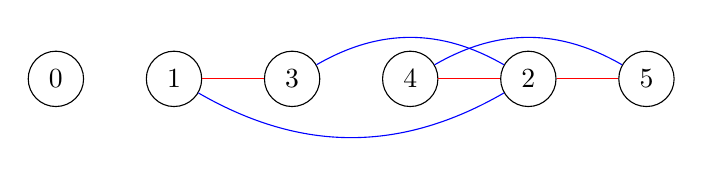
\begin{tikzpicture}
    	\begin{pgfonlayer}{nodelayer}
    		\node [style=node] (0) at (-3, 0) {0};
    		\node [style=node] (1) at (-1.5, 0) {1};
    		\node [style=node] (2) at (0, 0) {3};
    		\node [style=node] (3) at (1.5, 0) {4};
    		\node [style=node] (4) at (3, 0) {2};
    		\node [style=node] (5) at (4.5, 0) {5};
    	\end{pgfonlayer}
    	\begin{pgfonlayer}{edgelayer}
    		\draw [style=red edge] (1) to (2);
    		\draw [style=red edge] (3) to (4);
    		\draw [style=red edge] (4) to (5);
    		\draw [style=blue edge, bend right] (1) to (4);
    		\draw [style=blue edge, bend left] (2) to (4);
    		\draw [style=blue edge, bend left] (3) to (5);
    	\end{pgfonlayer}
    \end{tikzpicture}
    \caption{Breakpoint graph}
    \label{fig:breakpoint_graph}
\end{figure}

The red edges in the breakpoint graph identify the elements of $\pi$ that have to be split apart and the blue edges identify the elements of $\pi$ that have to be brought together (the missing adjacencies) in the process of sorting the permutation $\pi$. Figure \ref{fig:breakpoint_graph} shows the breakpoint graph of the permutation $(0\ 1\ 3\ 4\ 2\ 5)$.

An \textit{alternating cycle decomposition} of $G(\pi)$ is a collection of edge-disjoint alternating cycles, such that every edge of $G(\pi)$ is contained in exactly one cycle of the collection. We observe that for every breakpoint, a vertice in $G(\pi)$ must have a missing adjacency. And conversely, for every missing adjacency a vertex in $G(\pi)$ must have a breakpoint. Therefore, each vertex in our breakpoint graph has an equal number of incident red and blue edges.

\begin{corollary}
Hence, $G(\pi)$ can be decomposed into edge-disjoint alternating cycles.
\end{corollary}

The main result we prove in this section, relates the maximum number of alternating cycles of any cycle decomposition of $G(\pi)$ to the reversal distance of $\pi$.

First, we need to define some terminology. An alternating cycle in $G(\pi)$ is a \textit{$k$-cycle} if it has $k$ constituting red and $k$ constituting blue edges. We say, a reversal \textit{acts on} two red edges of $G(\pi)$ if those two red edges represent the breakpoints that are split apart by the reversal. Now, an alternating cycle in $G(\pi)$ is \textit{oriented} if there is a $1$- or a $2$-reversal acting on two constituting red edges. An alternating cycle of $G(\pi)$ is \textit{unoriented} if it is not oriented.

To give a more visual means of deducing whether an alternating cycle of $G(\pi)$ is oriented, we assign to each red edge $(\pi_i, \pi_{i+1})$ an orientation from $\pi_i$ to $\pi_{i+1}$, orienting red edges of $G(\pi)$ from the endpoint which appears first in $\pi$ to the endpoint which appears second. Then, we call an alternating cycle of $G(\pi)$ \textit{directed} with respect to $\pi$ if it is possible to walk along the whole cycle traversing each red edge in the direction of its orientation. An alternating cycle of $G(\pi)$ is called \textit{undirected} if it is not directed. For example, in figure \ref{fig:breakpoint_graph} the alternating cycle $(\{1,3\},\{2,3\},\{2,5\},\{4,5\},\{2,4\},\{1,2\})$ is directed with respect to $(0\ 1\ 3\ 4\ 2\ 5)$, whereas the alternating cycle $(\{1,3\},\{2,3\},\{2,4\},\{4,5\},\{2,5\},\{1,2\})$ is undirected with respect to $(0\ 1\ 3\ 4\ 2\ 5)$. \citeauthor*{Caprara1997} argues that an alternating cycle of $G(\pi)$ is oriented if and only if it is undirected \cite{Caprara1997}.

\begin{lemma}
\label{lem:1}
An oriented alternating cycle is a $2$-cycle if and only if the corresponding reversal acting on both red edges is a $2$-reversal.
\end{lemma}

\begin{proof}
Let $i \sim i'$ and $j \sim j'$. We observe that the $2$-cycles shown in figure \ref{fig:2cycles} are in fact the only types of $2$-cycles (with the exception of the symmetric case of an oriented $2$-cycle). Given an oriented $2$-cycle, we know that the corresponding reversal acting on its two constituting red edges brings $j'$ next to $j$ and $i$ next to $i'$, removing two breakpoints.

On the other hand, given a $2$-reversal $\rho$, we know that $\rho$ has to act on two red edges of $G(\pi)$. Identify with $k$ and $l$ the vertices incident to the first red edge and with $m$ and $n$ the vertices incident to the second red edge. Now, because $\rho$ is removes both red edges from the breakpoint graph, we know that either $k \sim m$ and $l \sim n$ or $k \sim n$ and $l \sim m$. Thus, forming a $2$-cycle in $G(\pi)$.
\end{proof}

\begin{figure}
    \begin{subfigure}[t]{.5\textwidth}
        \centering
        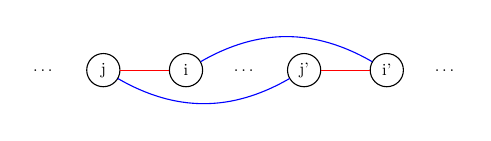
\begin{tikzpicture}[scale=0.6, every node/.style={scale=0.6}]
        	\begin{pgfonlayer}{nodelayer}
        		\node [style=node] (0) at (-1.25, 0) {i};
        		\node [style=node] (1) at (1.25, 0) {j'};
        		\node [style=node] (2) at (3, 0) {i'};
        		\node [style=node] (3) at (-3, 0) {j};
        		\node (4) at (0, 0) {$\dots$};
        		\node (5) at (-4.25, 0) {$\dots$};
        		\node (6) at (4.25, 0) {$\dots$};
        	\end{pgfonlayer}
        	\begin{pgfonlayer}{edgelayer}
        		\draw [style=blue edge, bend right] (3) to (1);
        		\draw [style=blue edge, bend left] (0) to (2);
        		\draw [style=red edge] (3) to (0);
        		\draw [style=red edge] (1) to (2);
        	\end{pgfonlayer}
        \end{tikzpicture}
        \caption{Oriented $2$-cycle}
        \label{fig:2reversal}
    \end{subfigure}
    \begin{subfigure}[t]{.5\textwidth}
        \centering
        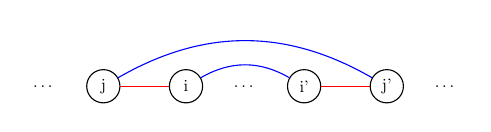
\begin{tikzpicture}[scale=0.6, every node/.style={scale=0.6}]
        	\begin{pgfonlayer}{nodelayer}
        		\node [style=node] (0) at (-1.25, 0) {i};
        		\node [style=node] (1) at (1.25, 0) {i'};
        		\node [style=node] (2) at (3, 0) {j'};
        		\node [style=node] (3) at (-3, 0) {j};
        		\node (4) at (0, 0) {$\dots$};
        		\node (5) at (-4.25, 0) {$\dots$};
        		\node (6) at (4.25, 0) {$\dots$};
        	\end{pgfonlayer}
        	\begin{pgfonlayer}{edgelayer}
        		\draw [style=blue edge, bend right] (2) to (3);
        		\draw [style=blue edge, bend left] (0) to (1);
        		\draw [style=red edge] (3) to (0);
        		\draw [style=red edge] (1) to (2);
        	\end{pgfonlayer}
        \end{tikzpicture}
        \caption{Unoriented $2$-cycle}
    \end{subfigure}
    \caption{$2$-cycles}
    \label{fig:2cycles}
\end{figure}

A similar lemma is proven by \citeauthor*{Christie1998} which we use as a corollary of this lemma in section \ref{sec:reversal_graph} \cite{Christie1998}.\padding

Let $c(\pi)$ denote the maximum number of alternating cycles in any alternating cycle decomposition of $G(\pi)$. \citeauthor*{Bafna1996} prove a fundamental theorem relating $b(\pi)$ with $c(\pi)$ \cite{Bafna1996}.

\begin{theorem}
\label{thm:1}
Let $\pi, \rho \in S_n$ and $\rho$ be a reversal. Then
\begin{align*}
    b(\pi) - b(\pi \circ \rho) + c(\pi \circ \rho) - c(\pi) \leq 1.
\end{align*}
\end{theorem}

\begin{figure}
    \begin{subfigure}[t]{.5\textwidth}
        \centering
        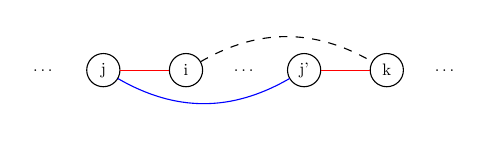
\begin{tikzpicture}[scale=0.6, every node/.style={scale=0.6}]
        	\begin{pgfonlayer}{nodelayer}
        		\node [style=node] (0) at (-1.25, 0) {i};
        		\node [style=node] (1) at (1.25, 0) {j'};
        		\node [style=node] (2) at (3, 0) {k};
        		\node [style=node] (3) at (-3, 0) {j};
        		\node (4) at (0, 0) {$\dots$};
        		\node (5) at (-4.25, 0) {$\dots$};
        		\node (6) at (4.25, 0) {$\dots$};
        	\end{pgfonlayer}
        	\begin{pgfonlayer}{edgelayer}
        		\draw [style=blue edge, bend right] (3) to (1);
        		\draw [style=red edge] (3) to (0);
        		\draw [style=red edge] (1) to (2);
        		\draw [style=dashed edge, bend left] (0) to (2);
        	\end{pgfonlayer}
        \end{tikzpicture}
        \caption{before reversal}
    \end{subfigure}
    \begin{subfigure}[t]{.5\textwidth}
        \centering
        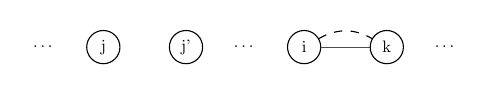
\begin{tikzpicture}[scale=0.6, every node/.style={scale=0.6}]
        	\begin{pgfonlayer}{nodelayer}
        		\node [style=node] (0) at (-1.25, 0) {j'};
        		\node [style=node] (1) at (1.25, 0) {i};
        		\node [style=node] (2) at (3, 0) {k};
        		\node [style=node] (3) at (-3, 0) {j};
        		\node (4) at (0, 0) {$\dots$};
        		\node (5) at (-4.25, 0) {$\dots$};
        		\node (6) at (4.25, 0) {$\dots$};
        	\end{pgfonlayer}
        	\begin{pgfonlayer}{edgelayer}
        		\draw [style=red edge] (1) to (2);
        		\draw [style=dashed edge, bend left] (1) to (2);
        	\end{pgfonlayer}
        \end{tikzpicture}
        \caption{after reversal}
    \end{subfigure}
    \caption{Case (i)}
    \label{fig:case_i}
\end{figure}

\begin{figure}
    \begin{subfigure}[t]{.5\textwidth}
        \centering
        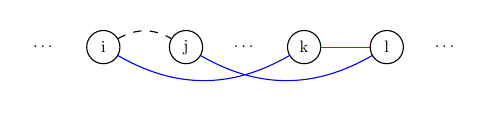
\begin{tikzpicture}[scale=0.6, every node/.style={scale=0.6}]
        	\begin{pgfonlayer}{nodelayer}
        		\node [style=node] (0) at (-3, 0) {i};
        		\node [style=node] (1) at (-1.25, 0) {j};
        		\node [style=node] (2) at (1.25, 0) {k};
        		\node [style=node] (3) at (3, 0) {l};
        		\node (4) at (0, 0) {$\dots$};
        		\node (5) at (-4.25, 0) {$\dots$};
        		\node (6) at (4.25, 0) {$\dots$};
        	\end{pgfonlayer}
        	\begin{pgfonlayer}{edgelayer}
        		\draw [style=blue edge, bend right] (0) to (2);
        		\draw [style=blue edge, bend right] (1) to (3);
        		\draw [style=red edge] (2) to (3);
        		\draw [style=dashed edge, bend left] (0) to (1);
        	\end{pgfonlayer}
        \end{tikzpicture}
        \caption{before reversal}
    \end{subfigure}
    \begin{subfigure}[t]{.5\textwidth}
        \centering
        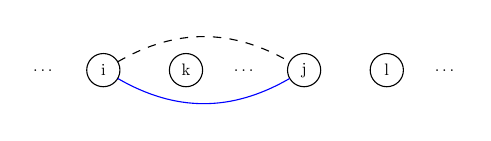
\begin{tikzpicture}[scale=0.6, every node/.style={scale=0.6}]
        	\begin{pgfonlayer}{nodelayer}
        		\node [style=node] (0) at (-3, 0) {i};
        		\node [style=node] (1) at (-1.25, 0) {k};
        		\node [style=node] (2) at (1.25, 0) {j};
        		\node [style=node] (3) at (3, 0) {l};
        		\node (4) at (0, 0) {$\dots$};
        		\node (5) at (-4.25, 0) {$\dots$};
        		\node (6) at (4.25, 0) {$\dots$};
        	\end{pgfonlayer}
        	\begin{pgfonlayer}{edgelayer}
        		\draw [style=blue edge, bend right] (0) to (2);
        		\draw [style=dashed edge, bend left] (0) to (2);
        	\end{pgfonlayer}
        \end{tikzpicture}
        \caption{after reversal}
    \end{subfigure}
    \caption{Case (ii)}
    \label{fig:case_ii}
\end{figure}

\begin{proof}
We consider each case $b(\pi) - b(\pi \circ \rho) \in [-2,2]$ separately.
\begin{enumerate}
    \item Let $b(\pi) - b(\pi \circ \rho) = 2$. Lemma \ref{lem:1} implies that a $2$-reversal $\rho$ removes a $2$-cycle from every alternating cycle decomposition of $G(\pi)$. Therefore, $c(\pi \circ \rho) - c(\pi) \leq -1$.
    \item Let $b(\pi) - b(\pi \circ \rho) = 1$. A $1$-reversal either creates one new adjacency (i) or creates two new adjacencies and simultaneously destroys one adjacency (ii).
        \begin{enumerate}[(i)]
            \item Let $j \sim j'$. Then figure \ref{fig:case_i} illustrates that every alternating cycle in $G(\pi \circ \rho)$ containing the edge $\{i,k\}$ induces an alternating cycle in $G(\pi)$ containing the edges $\{j,i\}$, $\{j,j'\}$, and $\{j',k\}$. Therefore, every alternating cycle decomposition of $G(\pi \circ \rho)$ into $c$ cycles induces an alternating cycle decomposition of $G(\pi)$ into $c$ cycles.
            \item Let $i \sim j$, $i \sim k$ and $j \sim l$. Then figure \ref{fig:case_ii} illustrates that every alternating cycle in $G(\pi \circ \rho)$ containing the edge $\{i,j\}$ induces an alternating cycle in $G(\pi)$ containing the edges $\{i,k\}$, $\{k,l\}$, and $\{j,l\}$. Therefore, every alternating cycle decomposition of $G(\pi \circ \rho)$ into $c$ cycles induces an alternating cycle decomposition of $G(\pi)$ into $c$ cycles.
        \end{enumerate}
    Therefore, for both subcases, $c(\pi \circ \rho) - c(\pi) \leq 0$ holds.
\end{enumerate}
Proof for other cases similar.
\end{proof}

Using \ref{thm:1}, \citeauthor*{Bafna1996} give a lower bound of the reversal distance of a permutation $\pi$ in terms of $b(\pi)$ and $c(\pi)$ \cite{Bafna1996}.

\begin{theorem}
\label{thm:2}
Let $\pi \in S_n$. Then
\begin{align*}
    d(\pi) \geq b(\pi) - c(\pi).
\end{align*}
\end{theorem}

\begin{proof}
Let $\pi_t = \pi, \pi_0 = id$ and $\rho_1, \dots, \rho_t$ a shortest sequence of reversals from $\pi_t$ to $\pi_0$. Then
\begin{align*}
    d(\pi_i) &= d(\pi_{i-1}) + 1 \\
             \overset{(\ref{thm:1})}&{\geq} d(\pi_{i-1}) + b(\pi_i) - b(\pi_{i-1}) + c(\pi_{i-1}) - c(\pi_i) \\[0.25cm]
    \iff & \begin{aligned}[t]
    d(\pi_i) - (b(\pi_i) - c(\pi_i)) &\geq d(\pi_{i-1}) - (b(\pi_{i-1}) - c(\pi_{i-1})) \\
                                     &\geq d(\pi_0) - (b(\pi_0) - c(\pi_0)) = 0
    \end{aligned}
\end{align*}
Setting $i=t$, proves the theorem.
\end{proof}

Using this lower bound, \citeauthor*{Bafna1996} already describe a $\frac{7}{4}$-approximation that is not considered in more detail here. \citeauthor*{Christie1998} was able to formulate a lower bound in terms of the number of $2$-cycles in a maximum alternating cycle decomposition \cite{Christie1998}.

\begin{lemma}
\label{lem:2}
Let $\mathcal{C}$ be a maximum alternating cycle decomposition of $G(\pi)$. Let $c_2(\pi)$ be the minimum number of alternating $2$-cycles in $\mathcal{C}$ and let $c_{3*}(\pi) = c(\pi) - c_2(\pi)$ be the remaining alternating cycles in $\mathcal{C}$.
Then
\begin{align*}
    c_{3*}(\pi) \leq \frac{1}{3}(b(\pi) - 2 c_2(\pi)).
\end{align*}
\end{lemma}

\begin{proof}
$b(\pi)$ is the number of red edges in $G(\pi)$ and $c_2(\pi)$ is the number of red edges in $2$-cycles of $G(\pi)$. Therefore, $b(\pi) - 2 c_2(\pi)$ is the number of \textit{free} red edges in $G(\pi)$ not occurring in $2$-cycles. $3 c_{3*}(\pi)$ is a lower bound to the number of red edges in $G(\pi)$ not occurring in $2$-cycles, proving the lemma.
\end{proof}

\begin{theorem}
\label{thm:3}
Let $\pi \in S_n$. Then
\begin{align*}
    d(\pi) \geq \frac{2}{3} b(\pi) - \frac{1}{3} c_2(\pi).
\end{align*}
\end{theorem}

\begin{proof}
Follows immediately from theorem \ref{thm:2} and lemma \ref{lem:2}.
\end{proof}

\section{3/2-approximation}
\label{sec:32_approximation}

In this section we discuss the $3/2$-approximation proposed by \citeauthor*{Christie1998} in detail \cite{Christie1998}. First, we describe how a sorting sequence of reversals can be obtained from an alternating cycle decomposition of $G(\pi)$ (section \ref{sec:reversal_graph}). In section \ref{sec:cycle_decomposition} we then describe how to find such a cycle decomposition. This then allows us to prove the approximation bound (section \ref{sec:approximation_bound}). Lastly, we describe the full algorithm and analyze its complexity respectively (section \ref{sec:algorithm}).

\subsection{Reversal graph}
\label{sec:reversal_graph}

To obtain a sorting sequence of reversals for a permutation $\pi$ given an alternating cycle decomposition $\mathcal{C}$ of its breakpoint graph $G(\pi)$, \citeauthor*{Christie1998} defines another graph.

\begin{definition}
Given an alternating cycle decomposition $\mathcal{C}$ of $G(\pi)$, the \textit{reversal graph} $R(\mathcal{C})$ is constructed as follows.

For each adjacency in $\pi$ we introduce an isolated blue vertex. For each $m$-cycle in $\mathcal{C}$ we introduce $m$ vertices, each representing a constituting blue edge. Each vertex $u$ represents the reversal $\rho(u)$ that acts on the two red edges incident to the blue edge. In the case of a $2$-cycle, two vertices in the reversal graph represent the same reversal. A vertex is colored red if the represented reversal is a $1$- or a $2$-reversal. Otherwise a vertex is colored blue.

Let $u$ be a vertex in $R(\mathcal{C})$. Define $l_b(u)$ and $r_b(u)$ to be the positions in $\pi$ of the leftmost and rightmost elements, respectively, that are incident to the blue edge in $G(\pi)$ represented by $u$. Similarly, $l_r(u)$ and $r_r(u)$ are defined to be the positions in $\pi$ of the leftmost and rightmost red edges that are adjacent to the blue edge represented by $u$. Hereby, the position of a red edge is the position of its leftmost incident vertex. Two vertices $u$ and $v$ are connected with an edge if $l_b(u) < l_b(v) < r_b(u) < r_b(v)$ or $l_b(v) < l_b(u) < r_b(v) < r_b(u)$ or $l_r(u) < l_r(v) < r_r(u) < r_r(v)$ or $l_r(v) < l_r(u) < r_r(v) < r_r(u)$.

Two cycles $C$ and $D$ \textit{interleave} if the reversal graph contains vertices $u$ and $v$ arising from $C$ and $D$ respectively, such that $\{u,v\}$ is an edge in $R(\mathcal{C})$. Blue edges \textit{interleave} in the breakpoint graph if the vertices representing them are adjacent in $R(\mathcal{C})$.
\end{definition}

\begin{figure}
    \centering
    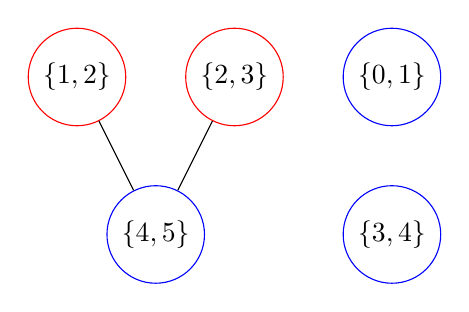
\begin{tikzpicture}
    	\begin{pgfonlayer}{nodelayer}
    		\node [style=red node] (0) at (0, 1) {$\{2,3\}$};
    		\node [style=red node] (1) at (-2, 1) {$\{1,2\}$};
    		\node [style=blue node] (2) at (-1, -1) {$\{4,5\}$};
    		\node [style=blue node] (3) at (2, -1) {$\{3,4\}$};
    		\node [style=blue node] (4) at (2, 1) {$\{0,1\}$};
    	\end{pgfonlayer}
    	\begin{pgfonlayer}{edgelayer}
    		\draw (0) to (2);
    		\draw (1) to (2);
    	\end{pgfonlayer}
    \end{tikzpicture}
    \caption{Reversal graph}
    \label{fig:reversal_graph}
\end{figure}

\begin{example}
Consider the alternating cycle decomposition
\begin{align*}
    \mathcal{C} = \{(&\{1,3\},\{2,3\},\{2,4\}, \\
                     &\{4,5\},\{2,5\},\{1,2\})\}
\end{align*}
of the breakpoint graph of $(0\ 1\ 3\ 4\ 2\ 5)$. The corresponding reversal graph is given in figure \ref{fig:reversal_graph}.
\end{example}

We observe that the only alternating cycle decomposition of $G(id)$ is $\mathcal{C} = \emptyset$. And therefore, the only reversal graph of the identity permutation $R(\emptyset)$ consists of $n+1$ isolated blue vertices. In the remainder of this chapter it our goal is to describe a way of transforming the reversal graph of a given alternating cycle decomposition into the reversal graph only consisting of isolated blue vertices with as few reversals as possible.

Let $u$ be a vertex of $R(\mathcal{C})$ representing reversal $\rho(u)$. Denote by $\mathcal{C}_u$ the alternating cycle decomposition of $G(\pi \circ \rho(u))$ that is obtained from $\mathcal{C}$ by removing one 2-cycle or shortening one of its cycles by one red edge and one blue edge.

The following lemma is given without proof.

\begin{lemma}
\label{lem:3}
$R(\mathcal{C}_u)$ can be derived from $R(\mathcal{C})$ by making the following changes to $R(\mathcal{C})$:
\begin{enumerate}
    \item flip the color of every vertex adjacent to $u$;
    \item flip the adjacency of every pair of vertices adjacent to $u$; and
    \item if $u$ is a red vertex, turn it into an isolated blue vertex.
\end{enumerate}
\end{lemma}

\begin{figure}
    \centering
    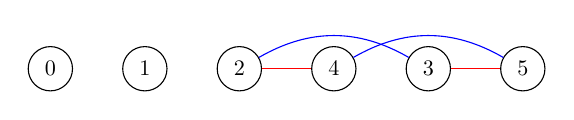
\begin{tikzpicture}[scale=0.8, every node/.style={scale=0.8}]
    	\begin{pgfonlayer}{nodelayer}
    		\node [style=node] (0) at (-3, 0) {0};
    		\node [style=node] (1) at (-1.5, 0) {1};
    		\node [style=node] (2) at (0, 0) {2};
    		\node [style=node] (3) at (1.5, 0) {4};
    		\node [style=node] (4) at (3, 0) {3};
    		\node [style=node] (5) at (4.5, 0) {5};
    	\end{pgfonlayer}
    	\begin{pgfonlayer}{edgelayer}
    		\draw [style=red edge] (2) to (3);
    		\draw [style=red edge] (4) to (5);
    		\draw [style=blue edge, bend left] (2) to (4);
    		\draw [style=blue edge, bend left] (3) to (5);
    	\end{pgfonlayer}
    \end{tikzpicture}
    \caption{Resulting breakpoint graph}
    \label{fig:breakpoint_graph_change}
\end{figure}

\begin{figure}
    \centering
    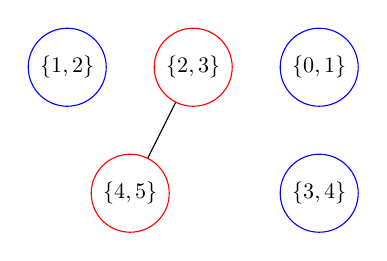
\begin{tikzpicture}[scale=0.8, every node/.style={scale=0.8}]
    	\begin{pgfonlayer}{nodelayer}
    		\node [style=red node] (0) at (0, 1) {$\{2,3\}$};
    		\node [style=blue node] (1) at (-2, 1) {$\{1,2\}$};
    		\node [style=red node] (2) at (-1, -1) {$\{4,5\}$};
    		\node [style=blue node] (3) at (2, -1) {$\{3,4\}$};
    		\node [style=blue node] (4) at (2, 1) {$\{0,1\}$};
    	\end{pgfonlayer}
    	\begin{pgfonlayer}{edgelayer}
    		\draw (0) to (2);
    	\end{pgfonlayer}
    \end{tikzpicture}
    \caption{Resulting reversal graph}
    \label{fig:reversal_graph_change}
\end{figure}

\begin{example}
Applying the reversal represented by vertex $\{1,2\}$ in figure \ref{fig:reversal_graph} results in the breakpoint and reversal graphs shown in figures \ref{fig:breakpoint_graph_change} and \ref{fig:reversal_graph_change} respectively.
\end{example}

\begin{corollary}
A reversal $\rho(u)$ affects only vertices that are in the same connected component as $u$.
\end{corollary}

We now prove a couple of lemmas that we use later.

\begin{lemma}
\label{lem:4}
$R(\mathcal{C})$ contains no isolated blue vertices arising from cycles in $\mathcal{C}$.
\end{lemma}

\begin{proof}
Omitted \cite{Christie1998}.
\end{proof}

The following is a simple consequence of the above lemma.

\begin{lemma}
\label{lem:5}
Vertices arising from an unoriented $2$-cycle of $\mathcal{C}$ must be in a connected component of $R(\mathcal{C})$ with vertices arising from at least one more alternating cycle of $\mathcal{C}$.
\end{lemma}

\begin{proof}
Let $u$ and $v$ represent the blue edges of an unoriented $2$-cycle of $\mathcal{C}$. Then its two constituting blue edges do not interleave. Hence, $R(\mathcal{C})$ does not connect $u$ and $v$ with an edge. If its constituting blue edges do not interleave with blue edges of any other alternating cycle of $\mathcal{C}$, then $u$ and $v$ would be isolated blue vertices. $\lightning$
\end{proof}

\begin{lemma}
\label{lem:6}
All vertices arising from the same alternating cycle in $\mathcal{C}$ are in the same connected component of $R(\mathcal{C})$.
\end{lemma}

\begin{proof}
Omitted \cite{Christie1998}.
\end{proof}

We call a connected component of $R(\mathcal{C})$ \textit{oriented} if it contains a red vertex or if it consists solely of an isolated blue vertex.

Let $A$ be a connected component of $R(\mathcal{C})$. We denote by $A_u$ the subgraph of $R(\mathcal{C}_u)$ that contains all the vertices of $A$. A sequence of reversals that turns the connected component $A$ of $R(\mathcal{C})$ into an isolated blue vertex, is called an \textit{elemination sequence} for $A$.

\begin{lemma}[\citeauthor*{Christie1998}]
\label{lem:7}
If a connected component $A$ of $R(\mathcal{C})$ is oriented and not an isolated blue vertex, it contains a red vertex $u$ such that $A_u$ is still oriented.
\end{lemma}

\begin{proof}
Omitted \cite{Christie1998}.
\end{proof}

With the above lemma we are now able to find an elimination sequence for the connected components of the reversal graph.

\begin{lemma}
\label{lem:8}
Let $A$ be an oriented connected component of $R(\mathcal{C})$ arising from $k$ different alternating cycles of $G(\pi)$. Then there is an elimination sequence for $A$ that contains $k$ $2$-reversals with all the other reversals being $1$-reversals.
\end{lemma}

\begin{proof}
As $A$ is oriented, we can use lemma \ref{lem:7} to repeatedly find a red vertex $u$ in $A$ such that $A_u$ is still oriented and apply $\rho(u)$.
By lemma \ref{lem:6}, we know that every vertex in $R(\mathcal{C})$ arising from an alternating cycle of $G(\pi)$ is contained within the same connected component. Therefore, every alternating cycle represented by vertices constituting $A$ eventually reduces to a $2$-cycle. Moreover, by lemma \ref{lem:1}, $\rho(u)$ is a $2$-reversal iff $u$ arises from an oriented $2$-cycle.

\end{proof}

\begin{lemma}
\label{lem:9}
Let $A$ be an unoriented connected component of $R(\mathcal{C})$ arising from $k$ different alternating cycles of $G(\pi)$. Then there is an elimination sequence for $A$ that contains one $0$-reversal, $k$ $2$-reversals, with all the other reversals being $1$-reversals.
\end{lemma}

\begin{proof}
Let $u$ be any blue vertex of $A$, then $\rho(u)$ is a $0$-reversal. By lemma \ref{lem:3}, $A_u$ is oriented.
Now, apply lemma \ref{lem:8} to obtain an elimination sequence for $A_u$.
\end{proof}

Using the elimination sequences we found for the connected components of $R(\mathcal{C})$ we are finally able to give an upper bound to the number of reversals we need to sort $\pi$.

\begin{theorem}
\label{thm:4}
Let $\pi \in S_n$ and $\mathcal{C}$ be an alternating cycle decomposition of $G(\pi)$. Then
\begin{align*}
    d(\pi) \leq b(\pi) - |\mathcal{C}| + u(\mathcal{C})
\end{align*}
where $u(\mathcal{C})$ is the number of unoriented components in $R(\mathcal{C})$.
\end{theorem}

\subsection{Cycle decomposition}
\label{sec:cycle_decomposition}

In this section our goal is to find an alternating cycle decomposition of $G(\pi)$. Motivated by the lower bound to the reversal distance in terms of $2$-cycles, we try to maximize the number of $2$-cycles in our cycle decomposition \cite{Christie1998}.

To find a large number of $2$-cycles in $G(\pi)$, \citeauthor*{Christie1998} constructs a new graph.

\begin{definition}
Given the permutation $\pi$, we construct the \textit{matching graph} $F(\pi)$ with vertices representing red edges in $G(\pi)$ and vertices $u, v$ being adjacent if they form a $2$-cycle in $G(\pi)$.
\end{definition}

We now observe that $2$-cycles of $G(\pi)$ are represented by edges in $F(\pi)$. We then find a maximum cardinality matching $M$ of $F(\pi)$. We call a $2$-cycle of $G(\pi)$ \textit{selected} if its corresponding edge of $F(\pi)$ is part of the matching $M$. Note, that we haven't yet found the set of edge-disjoint $2$-cycles that we need to construct an alternating cycle decomposition. This is because the matching ensures that all selected $2$-cycles are edge-disjoint on their red edges, but does not ensure that they are also edge-disjoint on their blue edges. To find a large set of edge-disjoint $2$-cycles, \citeauthor*{Christie1998} introduces another graph.

\begin{figure}
    \centering
    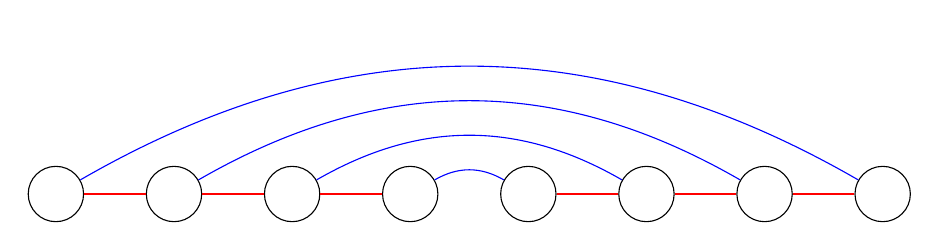
\begin{tikzpicture}
    	\begin{pgfonlayer}{nodelayer}
    		\node [style=node] (0) at (-4.5, 0) {};
    		\node [style=node] (1) at (-3, 0) {};
    		\node [style=node] (2) at (-1.5, 0) {};
    		\node [style=node] (3) at (0, 0) {};
    		\node [style=node] (4) at (1.5, 0) {};
    		\node [style=node] (5) at (3, 0) {};
    		\node [style=node] (6) at (4.5, 0) {};
    		\node [style=node] (7) at (6, 0) {};
    	\end{pgfonlayer}
    	\begin{pgfonlayer}{edgelayer}
    		\draw [style=red edge] (0) to (1);
    		\draw [style=red edge] (1) to (2);
    		\draw [style=red edge] (2) to (3);
    		\draw [style=red edge] (4) to (5);
    		\draw [style=red edge] (5) to (6);
    		\draw [style=red edge] (6) to (7);
    		\draw [style=blue edge, bend left] (3) to (4);
    		\draw [style=blue edge, bend left] (2) to (5);
    		\draw [style=blue edge, bend left] (1) to (6);
    		\draw [style=blue edge, bend left] (0) to (7);
    	\end{pgfonlayer}
    \end{tikzpicture}
    \caption{Ladder}
    \label{fig:ladder}
\end{figure}

\begin{definition}
Given a matching $M$, we construct the \textit{ladder graph} $L(M)$. $L(M)$ has a vertex for every $2$-cycle selected in $M$. Vertices form connected components when the represented $2$-cycles share a blue edge in $G(\pi)$. Such connected components of $L(M)$ are called \textit{ladders}. Figure \ref{fig:ladder} shows part of a breakpoint graph with $2$-cycles that form a ladder.

A selected $2$-cycle is called \textit{independent} if it is not part of a ladder. Otherwise it is called a \textit{ladder $2$-cycle}.
\end{definition}

As each $2$-cycle can share at most two blue edges with other $2$-cycles, the connected components of $L(M)$ are simple paths. Therefore, the set of $2$-cycles consisting of every other ladder $2$-cycle is edge-disjoint on all edges, resulting in the following theorem.

\begin{theorem}
\label{thm:5}
Given a maximum cardinality matching $M$ of $F(\pi)$ it is possible to find an alternating cycle decomposition $\mathcal{C}$ of $G(\pi)$ that contains at least $\left\lceil \frac{y}{2} \right\rceil$ ladder $2$-cycles and $z$ independent $2$-cycles.
\end{theorem}

\begin{proof}
Let $\mathcal{C}$ contain all independent $2$-cycles from $L(M)$ and every other alternate cycle of each ladder. Obtain the rest of $\mathcal{C}$ by adding any alternating cycle decomposition of the remaining unused edges of $G(\pi)$.
\end{proof}

Another lemma, \citeauthor*{Christie1998} shows, is given without proof.

\begin{lemma}
\label{lem:10}
Let $C$ be an unoriented ladder $2$-cycle in $\mathcal{C}$. Then the vertices of $R(\mathcal{C})$ that represent $C$ are part of a component that contains vertices representing an alternating cycle that is not a selected $2$-cycle.
\end{lemma}

\subsection{Approximation bound}
\label{sec:approximation_bound}

By theorem \ref{thm:3}, an algorithm that finds a sorting sequence of reversals of at most length $b(\pi) - \frac{1}{2} c_2(\pi)$ achieves an approximation bound of $\frac{3}{2}$.

\begin{theorem}
\label{thm:6}
Let $\pi \in S_n$. Then
\begin{align*}
    d(\pi) \leq b(\pi) - \frac{1}{2} c_2(\pi).
\end{align*}
\end{theorem}

\begin{proof}
Using theorem \ref{thm:5}, first find an alternating cycle decomposition $\mathcal{C}$ of $G(\pi)$ with at least $\left\lceil \frac{y}{2} \right\rceil$ ladder $2$-cycles and $z$ independent $2$-cycles.

Let $k$ be the number of $2$-cycles in oriented connected components of $R(\mathcal{C})$. Let $u$ be the number of unoriented connected components in $R(\mathcal{C})$ that include $l$ selected $2$-cycles and that, by lemma \ref{lem:10}, contain vertices representing remaining unselected $2$-cycles. Let $v$ be the number of remaining unoriented connected components consisting only of vertices representing $m$ independent selected $2$-cycles.

Note that $\mathcal{C}$ has at least $k+l+u+m$ alternating cycles and $R(\mathcal{C})$ has $u+v$ unoriented connected components.

By theorem \ref{thm:4}, we can now sort $\pi$ using at least $k+l+u+m$ $2$-reversals and only $u+v$ $0$-reversals. Therefore
\begin{align*}
    d(\pi) &\leq b(\pi) - k - l - u - m + u + v \\
           &= b(\pi) - k - l - m + v.
\end{align*}
All that is left to show is $k+l+m-v \geq \frac{1}{2} c_2(\pi)$. We know:
\begin{enumerate}
    \item $l+m$ is the number of selected $2$-cycles in unoriented connected components of $R(\mathcal{C})$. $k$ is the total number of $2$-cycles in oriented connected components of $R(\mathcal{C})$. As $\left\lceil \frac{y}{2} \right\rceil + z$ is the number of selected $2$-cycles in $\mathcal{C}$, $k+l+m \geq \left\lceil \frac{y}{2} \right\rceil + z$ holds.
    \item As each connected components of $R(\mathcal{C})$ counted by $v$ represents at least one unoriented $2$-cycle, lemma \ref{lem:5} implies that such a connected component must also represent at least one more alternating cycle in $\mathcal{C}$. As the connected component only represents independent $2$-cycles, we know that it must represent at least two independent $2$-cycles. As $z$ is the number of independent $2$-cycles, $v \leq \left\lfloor \frac{z}{2} \right\rfloor$ holds.
    \item As the set of selected $2$-cycles is not necessarily edge-disjoint, $|M| = y+z \geq c_2(\pi)$.
\end{enumerate}
And therefore
\begin{align*}
    k+l+m-v &\geq \left\lceil \frac{y}{2} \right\rceil + z - v                                          & (1) \\
            &\geq \left\lceil \frac{y}{2} \right\rceil + z - \left\lfloor \frac{z}{2} \right\rfloor     & (2) \\
            &= \left\lceil \frac{y}{2} \right\rceil + \left\lceil \frac{z}{2} \right\rceil \\
            &\geq \frac{1}{2} c_2(\pi).                                                                 & (3)
\end{align*}
\end{proof}

\subsection{Algorithm}
\label{sec:algorithm}

The approximation algorithm with a performance ratio of $\frac{3}{2}$, is outlined in the following.

\begin{algorithm}
    \SetKwInOut{Input}{Input}
    \Input{permutation $\pi \in S_n$}
    construct the matching graph $F(\pi)$\;
    find a maximum cardinality matching $M$ for this graph\;
    construct alternating cycle decomposition $\mathcal{C}$ using this matching\;
    construct the reversal graph $R(\mathcal{C})$\;
    find an elimination sequence for $R(\mathcal{C})$\;
    \caption{Approximation algorithm \cite{Christie1998}}
\end{algorithm}

The matching graph can be constructed in $O(n)$ time. The maximum cardinality matching can be obtained from $F(\pi)$ using the algorithm of Micali and Vazirani in $O(|V||E|^{\frac{1}{2}})$ time \cite{Micali1980} where $|V|$ and $|E|$ are the number of vertices and edges respectively. Therefore, it is possible to find such a matching in $O(n^{\frac{3}{2}})$ time. The alternating cycle decomposition can be obtained from the matching in $O(n)$ time. The reversal graph can be constructed in $O(n^2)$ time. The algorithm to find an elimination sequence of $R(\mathcal{C})$ is outlined below and terminates in $O(n^4)$ time. So the overall time-complexity of the algorithm is $O(n^4)$ \cite{Christie1998}. Using results from \citeauthor*{Kaplan1997}, the time-complexity can be improved to $O(n^2)$ \cite{Kaplan1997}.

\begin{algorithm}
    \SetKwInOut{Input}{Input}
    \Input{reversal graph $R(\mathcal{C})$}
    for each unoriented connected component, apply a reversal represented by a blue vertex\;
    \While{not sorted $\pi$}{
        u := first red vertex\;
        found := false\;
        \While{not found}{
            apply $\rho(u)$ to get $\mathcal{C}_u$\;
            generate $R(\mathcal{C}_u)$\;
            count unoriented connected components in $R(\mathcal{C}_u)$\;
            \eIf{there are no unoriented connected components}{
                found := true\;
            }{
                u := next red vertex\;
            }
        }
    }
    \caption{Finding an elimination sequence \cite{Christie1998}}
\end{algorithm}

\section{Conclusion}
\label{sec:conclusion}

We have seen multiple layers of abstraction that allowed us to describe a $3/2$-approximation. As was mentioned in the introduction, a better but more complex approximation was obtained later by \citeauthor*{Berman2001}.

An interesting property of the discussed $3/2$-approximation is that when constructing the alternating cycle decomposition, any cycle decomposition of the edges that are not part of $2$-cycles will suffice \cite{Christie1998}.

\printbibliography

\end{document}
